\documentclass{article}

\usepackage{../preamble}
\standalonetrue

\pagestyle{fancy}
\fancyhf{}
\rhead{Section \thesection}
\lhead{PHYS 304 Lecture 3}
\rfoot{Page \thepage}


\title{PHYS 304 Lecture 3}
\author{Ashtan Mistal}
\date{!!!}

\begin{document}

\ifstandalone
\maketitle
\fi

\graphicspath{{./Lecture03/}}

\section{Review of Key Points From Last Day}

Classically, we can calculate the position of a particle at all times, x(t) (and hence know precisely all the information possible about its dynamics), using Newton’s equation of motion, knowing the particle’s position and velocity at specified times , and the force field acting on the particle.

Quantum mechanically, the most complete calculation of a particle’s dynamics involves solving Schrodinger's equation for the particle’s (complex) wavefunction,$ \Psi(x,t)$, given the force field and the wavefunction at some time $t_0$. 


$$\int_a^b |\Psi(x,t)|^2 dx = \left\{ \text{Probability of finding the particle between } a \text{ and } b \text{, at time } t \right\}$$

In classical mechanics, $x(t)$ is a dynamical variable where x represents the position of the centre of mass of the particle.  In quantum mechanics, $x$ is not a function of $t$, and is merely a parameter representing a cartesian coordinate in space.


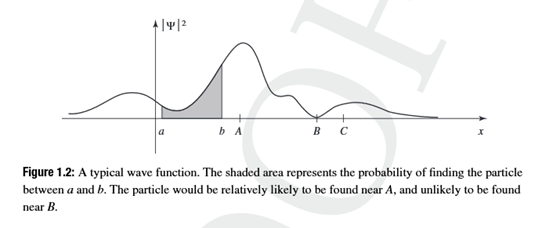
\includegraphics[width = 0.7 \textwidth]{Lecture02/2.png}

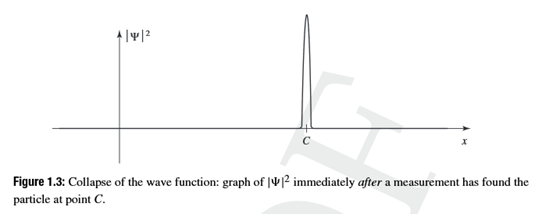
\includegraphics[width = 0.7 \textwidth]{Lecture02/3.png}

The act of measurement changes the wavefunction (in general).

This makes sense, since doing a measurement involves applying some “additional” potentials not included in how one would have used to solve for the wavefunction before the measurement.

\subsection*{Today's Activities}

\begin{enumerate}
    \item Develop some intuition for the relationship between wave-like and particle-like behaviours
    \item Introduce a measure of the degree of “localization” of a wave function
    \item An intuitive derivation of “the momentum” associated with a wavefunction
    \item Bi-weekly quiz (4:40-4:50 on Canvas)
\end{enumerate}

\section{Particle and wave concepts}

\subsection{Activity 1}

Viewing videos https://youtu.be/jcXF1jvhMx4 (example 1)

and https://www.youtube.com/watch?v=MBSZcCT0wvA

(example 3)

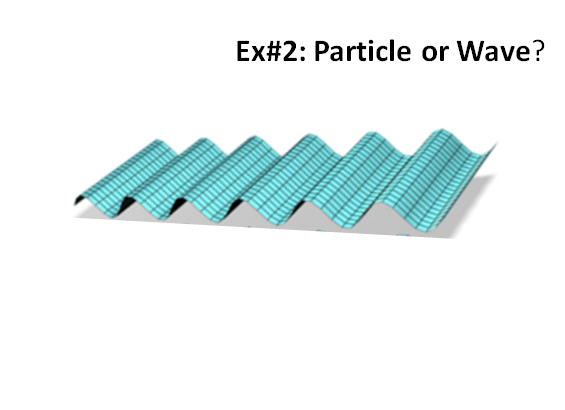
\includegraphics[width = 0.6 \textwidth]{Lecture03/1.png}

Of course, they are all waves and particles in quantum mechanics. But intuitively, the first one is straightforward, and the second one is also straightforward. For the second one, visualize it moving, time averaged, same everywhere in space. The third is a random superposition of waves. 

Asked class if anyone can relate 1 and 3. It is a classical particle represented by a coherent superposition of many waves with different wavelengths -- a wavepacket. 

Spent time digging deeper into the following:

\begin{itemize}
    \item Sketching the magnitude and phase of $\Psi(x,y,t)$ for each case. Note the subtleties: case 1 and 3 give the magnitude of $\Psi^2(x,y,t)$ with the video giving the time dimension. Case 2 is ambiguous (no axes, static picture). It could be $\Psi(x,y)$ at a fixed time $t$, or it could also be $\text{Re} \left( \Psi(x,y) \right)$ at a fixed $t$, or $\text{Re} \left( \Psi(x,t) \right)$ for a fixed $y$. Let's assume it is the former for now. What is the key parameter that makes one choose "particle-like" versus "wave-like" behaviour? Again, the answer to this is subtle: when we see the the video (noting the time dependence), then it is the fact that the particle remains localized as it moves in case 1, whereas it is delocalized in case 3. 
    \item Case 2 and case 3 are most similar -- think about how tehy are related. 
\end{itemize}

\subsection*{What happens when you add waves?}

Showed the PHET Fourier simulation. Key points:

\begin{itemize}
    \item plane wave is “perfect” wave, i.e. infinitely and uniformly delocalized $(\Psi^2)$, and characterized by a wavelength $\lambda$
    \item Adding plane different waves with different wavelengths introduces some degree of non-uniformity in $\Psi^2$ (SUM OF WAVES) SQUARED, NOT SUM OF (WAVES SQUARED)
    \item Depending critically on the relative phase and range of different wavelength waves, the sum can in some cases be made to resemble a localized particle
    \item Could(?) use this to introduce the uncertainty principle here (where just quote result, in terms of delta x and delta lambda, not delta p, and emphasize the equality only occurs in the limit (typically associated with a particle-like wavefunction.  Example 1 likely nearly at the equality point, example 3 far off.  
\end{itemize}

\subsection{Activity 2 and 3}

Using probability distributions, e.g. $|\Psi(x,t)|^2$

\begin{enumerate}
    \item What value must $\int_{- \infty}^{\infty} |\Psi(x,t)|^2 dx$ be for any wave function? ans: 1
    \item Give a physical interpretation. \textit{Unity, since the particle must be somewhere, so adding up all the probabilities of finding it where it might possibly be must equal unity.}
\end{enumerate}

What physical interpretation would you give to the following integral involving some function f(x), if $f(x)=x$? (provide an explanation for your answer): $\int_{-\infty}^\infty f(x) |\Psi(x,t)|^2 dx $
\textit{This is the average value you might measure if you had multiple copies of the same wavefunction and measured it several times, getting, in general, a different value of the particle’s location each time you measured it. Or, if you had an ensemble of identical wavefunctions and measured them all, and plotted the various locations x that you measured from each member of the ensemble, this would be the average value measured.}

\subsection{Activity 4}

What would you replace $f(x)$ by in the integral of Q3, if you wanted a measure of the “size of”, or the “delocalization of” the particle associated with the wavefunction $\Psi(x,t_0)$ ?  (as always, provide an explanation for your answer)

\textit{$(\text{x - the average value of x})^2$ or $\Delta x^2$}

$$\langle \Delta x^2 \rangle = \int_{- \infty}^\infty (x - \langle x \rangle)^2 |\Psi(x,t_0)|^2 dx$$

Why not $x - \langle x \rangle$? Because it's zero, and adding absolute value signs is not mathematically convenient, thus it's better to square it. Draw a distribution, and note that the "distance" from the mean is $x - \langle x \rangle$

If we draw 1 dimensional time slices of localized wavepacket probability distribution as it moves for different times (noting that $\langle x \rangle$ varies with time), so we differentiate to get an estimate of momentum. Does this give the distribution of the momenta values you might get when you measure the particle's momentum? no. 

\subsection{Activity 5}

How might you go about finding the “expectation value” (really the average value) of the particle’s momentum that you would measure if it is in state $\Psi(x,t)$?  Hint: you know how to calculate $\langle x \rangle (t)$. 

$$\frac{d \langle x \rangle (t)}{dt}$$

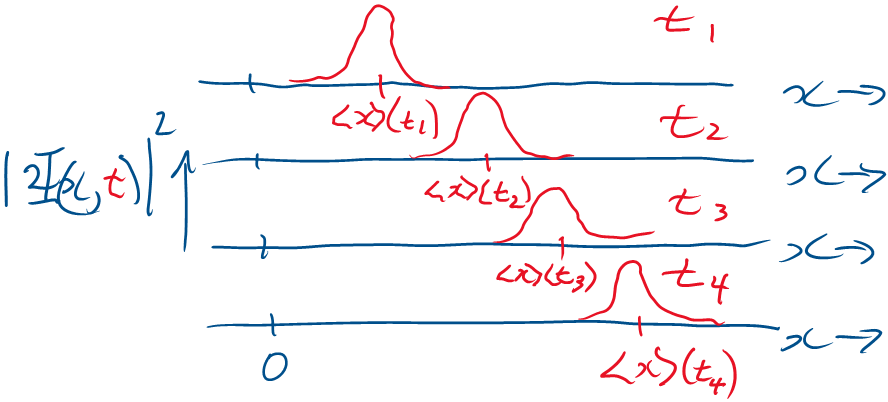
\includegraphics[width = 0.6 \textwidth]{Lecture03/2.png}


\subsection{Activity 6}

Write an expression for how to calculate the expectation value of a particle’s total energy (kinetic plus potential) using the following:

$$\langle Q(x,p) \rangle = \int \Psi^* \left[ Q(x, -i \hbar \frac{\partial}{\partial x} \right] \Psi dx$$

General algorithm for finding the expectation value of some observable property that can be classically expressed in terms of p and x:

\begin{enumerate}
    \item Write the classical expression for the quantity of interest in terms of p and x (eg: total energy = $\frac{p^2}{2m} + V(x)$
    \item Substitute $- \hbar \frac{\partial}{\partial x}$ for all p's and x for all x's
    \item Insert this as the operator $\left[ Q(x, -i \hbar \frac{\partial}{\partial x} \right]$ in the above equation. (between $\Psi^*$ and $\Psi$). 
\end{enumerate}




\end{document}